\section{Bottom-up syntax analysis}

To systematically construct a bottom-up syntax analyzer we have: 
\begin{enumerate}
    \item Construction of the pilot graph: the pilot drives the bottom-up syntax analyzer. 
        In each macro-state the pilot incorporates all the information about any possible phrase form that reaches the m-state (with look-ahead). 
        Each m-state contains machine states with look-ahead, which are the characters we expect to see in the input at reduction time.
    \item The $m$ states are used to build a few analysis threads in the stack, which correspond to possible derivations: computations of the machine network, or paths with $\varepsilon$-arcs at each machine change, labeled with the scanned string. 
    \item Verification of determinism conditions on the pilot graph: shift-reduce conflicts, reduce-reduce conflicts, and convergence conflicts. 
    \item If the determinism test is passed, the bottom-up syntax analyzer can analyze the string deterministically.
    \item The bottom-up syntax analyzer uses the information stored in the pilot graph and in the stack. 
\end{enumerate}

\begin{definition}
    The \emph{set of initials} is the set of chars found starting from state $q_A$ of machine $M_A$ of the net $M$: 
    \[\textnormal{Ini}(q_A)=\textnormal{Ini}(L(q_A))=\{a \in \Sigma|a\Sigma^{*}\cap L(q_A) \neq \varnothing\}\]
\end{definition}
The elements of the initial set are defined in three possible cases: 
\begin{itemize}
    \item $a \in \textnormal{Ini}(q_A)$ if exists an arc $q_A \overset{a}{\rightarrow}r_A$. 
    \item $a \in \textnormal{Ini}(q_A)$ if exists an arc $q_A \overset{B}{\rightarrow}r_A$ and $a \in \textnormal{Ini}(0_B)$. 
    \item $a \in \textnormal{Ini}(q_A)$ if exists an arc $q_A \overset{B}{\rightarrow}r_A$ and $L(0_B)$ is nullable and $a \in \textnormal{Ini}(r_A)$.
\end{itemize}
\begin{example}
    Consider the following grammar: 
    \[
    \begin{cases}
        S \rightarrow Aa \\
        A \rightarrow BC \\
        B \rightarrow b|\varepsilon \\
        C \rightarrow c|\varepsilon
    \end{cases}    
    \]
    The corresponding machine net is: 
    \begin{figure}[H]
        \centering
        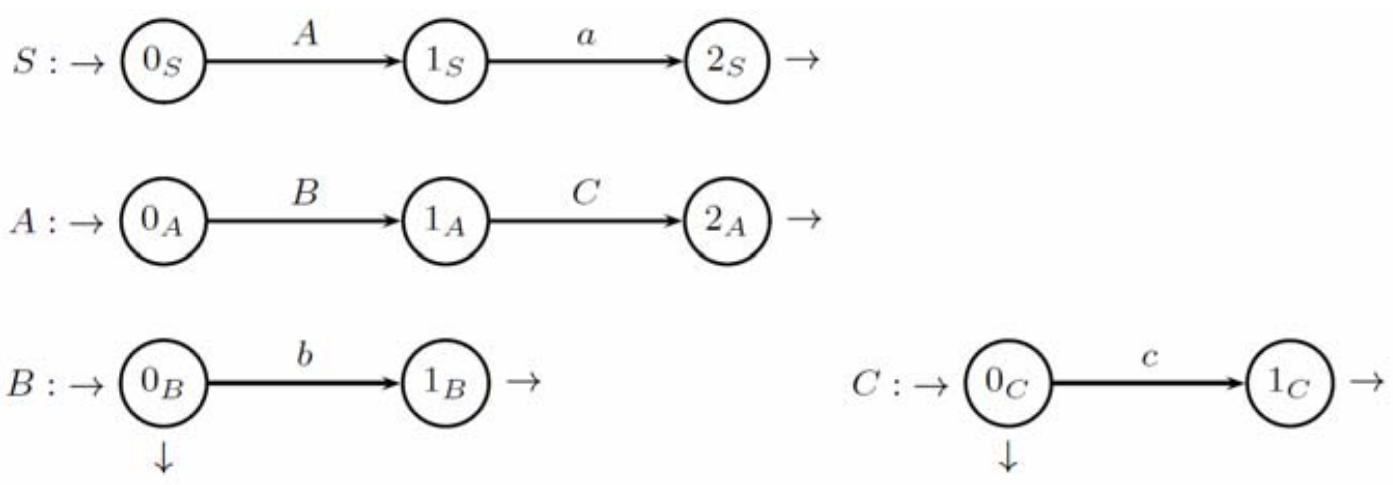
\includegraphics[width=0.5\linewidth]{images/net1.png}
    \end{figure}
    To find the set of initials for $S_0$ we have to check the following states: 
    \begin{itemize}
        \item $\textnormal{Ini}(0_S)=\textnormal{Ini}(0_A) \cup \textnormal{Ini}(1_S)$ because $L(0_A)$ is nullable. 
        \item $\textnormal{Ini}(0_A)=\textnormal{Ini}(0_B) \cup \textnormal{Ini}(1_A)$ because $L(0_B)$ is nullable. 
        \item $\textnormal{Ini}(1_A)=\textnormal{Ini}(0_C) \cup \textnormal{Ini}(2_A)$ because $L(0_C)$ is nullable. 
    \end{itemize}
    The final result is: 
    \[\textnormal{Ini}(0_S)=\{b\} \cup \{c\} \cup \{a\}\]
\end{example}

\begin{definition}
    An \emph{item} is: 
    \[\left\langle q_B,a\right\rangle \textnormal{ in } Q \times (\Sigma \cup \{\dashv\})\]
\end{definition}
Two or more items with the same state can be grouped into one item. 
An item with a machine final state is said to be a reduction item. 

\begin{definition}
    The function \emph{closure} computes a kind of closure of a set $C$ of items with look-ahead. 
\end{definition}
To find the closure of $C$ we have to apply this recursive clause until a fixed point is reached (the initial setting is $\textnormal{closure}(C)=C$): 
\[
    \left\langle 0_B,b\right\rangle \in \textnormal{closure}(C) \textnormal{ if }
    \begin{cases}
        \exists \textnormal{ candidate } \left\langle q,a\right\rangle \in C \textnormal{ and} \\
        \exists \textnormal{ arc } q \overset{B}{\rightarrow} r \textnormal{ in } \mathcal{M} \textnormal{ and} \\
        b \in \textnormal{Ini}(L(r)a)
    \end{cases}
\]
\begin{definition}
    The \emph{shift operation} is defined as: 
    \[
    \begin{cases}
        \theta(\left\langle p_A,\rho\right\rangle,X)=\left\langle q_A,\rho\right\rangle \textnormal{ if the arc } p_a \overset{X}{\rightarrow} q_a \textnormal{ exists} \\
        \textnormal{The empty set otherwise}
    \end{cases}    
    \]
\end{definition}
A shift corresponds to a transition in a machine $Y$: 
\begin{itemize}
    \item if $X = c$ is a terminal symbol, then shift is a bottom-up syntax analyzer move that reads a char $c$ in the input. 
    \item If $X$ is a non-terminal symbol, then shift is a bottom-up syntax analyzer $\varepsilon$-move after a reduction $z \rightarrow X$, and it does not read any input.
    \item Machine $Y$ runs a transition with nonterminal label $X$. 
    \item The analysis goes on after recognizing an input substring $z \in L (X)$ derivable from the nonterminal $X$. 
\end{itemize}
The shift operation extends to sets of items (denoted as m-state): 
\[\vartheta(C,X)=\bigcup_{\forall \gamma \in C} \vartheta(\gamma,x)\]

\subsection*{Pilot graph}
\begin{definition}
    The \emph{pilot graph} is a deterministic finite state automaton, named $\mathcal{P}$, defined by the following entities:
    \begin{itemize}
        \item The set $R$ of m-states. 
        \item The pilot alphabet is the union $\Sigma\cup V$ of the terminal and non-terminal alphabets, to be also named the grammar symbols.
        \item The initial m-state, $I_0$, is the set $I_0=closure(\left\langle 0_S,\dashv \right\rangle )$. 
        \item The m-state set $R={I_0,I_1,\dots}$ and the state-transition function $\theta:R \times (\Sigma \cup V) \rightarrow R$ are computed starting from $I_0$. 
    \end{itemize}
\end{definition}
The construction of the pilot graph is incremental: it ends when nothing changes any longer. 
It has no final states since it does not recognize strings. 
The item in each m-state $I$ of the pilot are parted into two groups: 
\begin{itemize}
    \item Base: contains the items obtained after a shift, which are non-initial states.
    \item Closure: contains the items obtained after a closure, which are initial states.
\end{itemize}
\begin{definition}
    The \emph{kernel} of an m-state $I$ is the set of the m-states of $I$ without look-ahead. 
\end{definition}
\begin{algorithm}[H]
    \caption{Pilot graph construction algorithm}
        \begin{algorithmic}[1]
            \State $R^{'} \leftarrow \{I_0\}$
            \While {$R \neq R^{'}$}
                \State $R \leftarrow R^{'}$
                \For {each m-state $I \in R$ and symbol $X \in \Sigma \cup V$}
                    \State $I^{'} \leftarrow \textnormal{closure}(\vartheta(I,X))$
                    \If {$I^{'} \neq \varnothing$}
                        \State add arc $I \overset{X}{\rightarrow} I^{'}$ to the graph of $\vartheta$
                        \If {$I^{'} \notin R$}
                            \State add m-state $I^{'}$ to the set $R^{'}$
                        \EndIf
                    \EndIf
                \EndFor
            \EndWhile
        \end{algorithmic}
\end{algorithm}
\begin{example}
    Consider the grammar: 
    \[
    \begin{cases}
        E \rightarrow T^{*} \\
        T \rightarrow '('E')'|a
    \end{cases}
    \]
    The corresponding machine net is: 
    \begin{figure}[H]
        \centering
        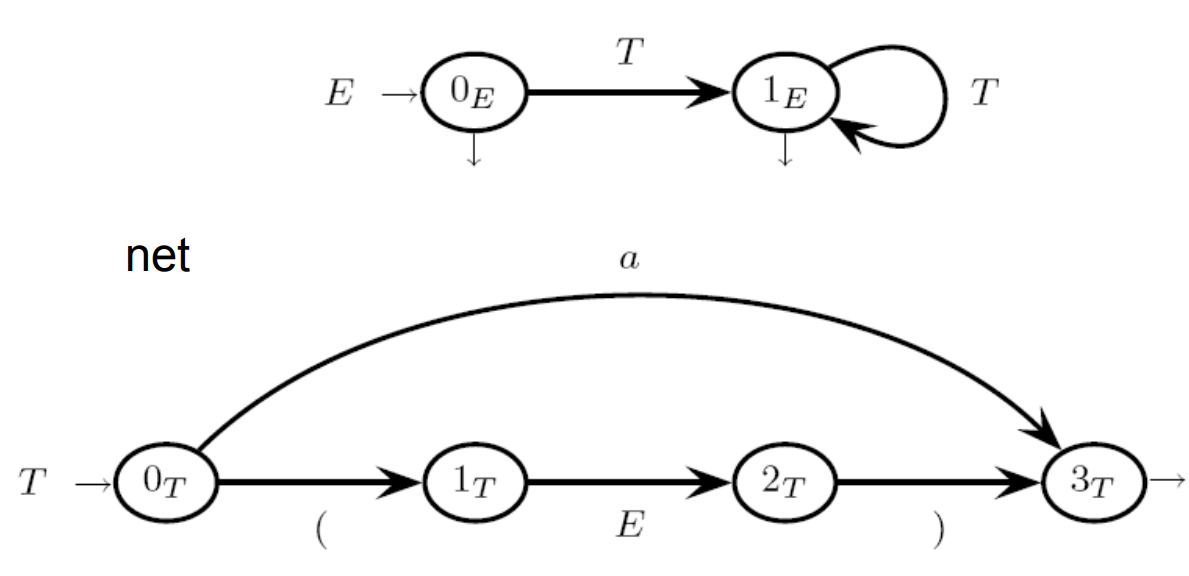
\includegraphics[width=0.5\linewidth]{images/net2.png}
    \end{figure}
    By applying the previous algorithm we obtain the following pilot graph: 
    \begin{figure}[H]
        \centering
        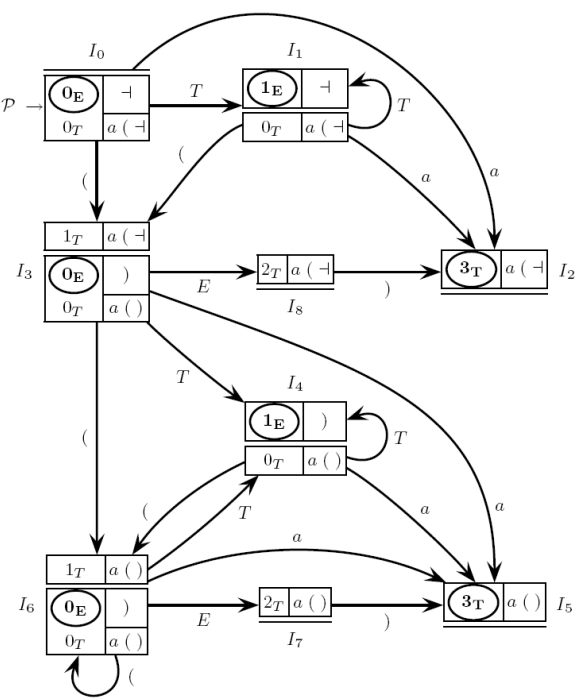
\includegraphics[width=0.5\linewidth]{images/pil.png}
    \end{figure}
    It is possible to note that the kernel-equivalent m-states are: 
    \[(I_3, I_6),(I_1, I_4),(I_2, I_5),(I_7, I_8)\]
\end{example}
If an m-state contains an item with a final state, then the bottom-up syntax analyzer makes a reduction move. 
The look-ahead of the reduction item indicates the input characters expected at reduction time. 
The bottom-up syntax analyzer verifies the current input char $cc$, and: 
\begin{itemize}
    \item If $cc \in \textnormal{look-ahead}$, bottom-up syntax analyzer makes a reduction.
    \item Else bottom-up syntax analyzer reads input char $cc$, and makes a shift on an arc with label $cc$.
    \item Otherwise, bottom-up syntax analyzer stops and rejects.
\end{itemize}

\subsection*{ELR(1) method}
The condition for allying the ELR(1) method are to not have: 
\begin{itemize}
    \item Shift-reduce conflicts: exists a reduction item with look-ahead that overlaps with the terminal symbols on the outgoing arcs. 
        If there are some conflicts of this type the bottom-up syntax analyzer is unable to choose between shift and reduction. 
    \item Reduce-reduce conflicts: exists two or more reduction items with look-ahead that overlap. 
        If there are some conflicts of this type the bottom-up syntax analyzer is unable between the two possible reductions. 
    \item Convergence conflicts: an m-state contains two or more items such that their two or more next states are defined for a symbol X (terminal or not). 
        If there are some conflicts of this type the bottom-up syntax analyzer is unable the reduction between the reductions of the converging paths. 
\end{itemize}
\begin{definition}
    A multiple transition is \emph{convergent} if: 
    \[\delta(p,X)=\delta(r,X)\]

    A multiple convergent transition has a \emph{conflict} if: 
    \[\pi \cap \rho \neq \varnothing\]
\end{definition}

\subsection*{Bottom-up syntax analyzer's workflow}
The bottom-up syntax analyzer follows this workflow: 
\begin{enumerate}
    \item The bottom-up syntax analyzer scans a string and executes a sequence of shift and reduction moves.
    \item The bottom-up syntax analyzer pushes groups of items and starts from those in the initial pilot m-state.
    \item Each m-state item becomes a 3-tuple by adding to it a backward-directed pointer that helps to reconstruct the different analysis threads constructed in parallel.
    \item The bottom-up syntax analyzer decides whether to scan or reduce basing on the look-ahead in the pilot.
    \item If the condition ELR (1) is satisfied, then the bottom-up syntax analyzer is deterministic. 
\end{enumerate}
Note that the length of the reduction handle is not fixed and so a rule  may generate phrases of unbounded length. 
The reduction handle length is determined at reduction time by using the pointers.
The pointer chain is followed backwards unto where the analysis thread started.
A pointer value $\perp$ identifies a thread start point and all the closure items have a pointer value $\perp$, so these items are the start points of new threads. 
A 3-tuple with pointer different from $\perp$ continues an already started thread; the pointers different from $\perp$ are displayed as $\#i$; a pointer value $\#i$ means that the pointer is targeted to the $i$-th item (from top to bottom) in the previous stack element. 

\subsection*{Computational complexity}
When analyzing a string $x$ of length $n = \left\lvert x \right\rvert $, the number of elements in the stack is greater or equal to $(n + 1)$. 
To count the number of bottom-up syntax analyzer moves, we consider this contributes: 
\begin{itemize}
    \item Number of terminal shift, denoted as $n_T$. 
    \item Number of nonterminal shift, denoted as $n_N$. 
    \item Number of reductions, denoted as $n_R$. 
\end{itemize}
These variables are linked in the following ways: the terminal shift corresponds to the length of the string and the number of nonterminal shift is the same as the number of reductions. 
As a result, we have that the total number of bottom-up syntax analyzer moves is: 
\[n_T+n_N+n_R=n+2n_R\]
Furthermore: 
\begin{itemize}
    \item The number of reductions with one or more terminals ($A \rightarrow a$) is less or equal to $n$. 
    \item The number of reductions of type null ($A \rightarrow \varepsilon$) and copy ($A \rightarrow B$) is linearly bounded by $n$. 
    \item The number of reductions without any terminals ($A \rightarrow BC$) is linearly bounded by $n$.
\end{itemize}
As a result we have that the final time complexity is $O(n) \leq kn+c$ for some integer constants $k$ and $c$. 
Furthermore, the space complexity is the max stack size, which is $n_T+n_N \leq kn+c$. 
It is important to note that the space complexity is always upper-bounded by time complexity. 

\subsection*{Bottom-up syntax analyzer implemented with a vectored stack}
In an implementation of the bottom-up syntax analyzer with some programming language we can always mine the stack elements underneath the top one and directly look deep inside the stack. 
The third field of a stack item can be an integer that directly points back to the position of the stack element where the analysis thread begins. 

Actually the analyzer is no longer a true bottom-up syntax analyzer as the stack alphabet becomes infinite.
Such a variation is possible in every analyzer of practical interest and is not costly.
In a closure item, write the current stack element index instead of the initial value $\perp$.
In a base item, copy the same index value as that in the item before.
So the bottom-up syntax analyzer does not scan back the reduction handle and goes directly to the origin.